\documentclass[12pt]{article}

%Russian-specific packages
%--------------------------------------
\usepackage[T2A]{fontenc}
\usepackage[utf8]{inputenc}
\usepackage[english, russian]{babel}
%for search in russian
\usepackage{cmap}
%--------------------------------------

%Math-specific packages
%--------------------------------------
\usepackage{amsmath}
\usepackage{amssymb}

%Format-specific packages
%--------------------------------------
\usepackage[left=2cm,
            right=2cm,
            top=1cm,
            bottom=2cm,
            bindingoffset=0cm]{geometry}

\usepackage{amsthm}
\newtheorem{lemma}{Лемма}
\newtheorem{definition}{Определение}
\newtheorem*{remark}{Замечание}

\def\LCS{
    \mathrm{LCS}
}

\usepackage{tikz}
\usepackage{pgfplots}

\usetikzlibrary{matrix, tikzmark, calc, trees, positioning,arrows,fit,shapes}
\tikzset{
table/.style={
  matrix of nodes,
  row sep=-\pgflinewidth,
  column sep=-\pgflinewidth,
  nodes={draw, rectangle,text width=2em,align=center},
  text depth=1.25ex,
  text height=2.5ex,
  text width=1.5ex,
  nodes in empty cells
},
row 1/.style={nodes={fill=green!10}},
column 1/.style={nodes={fill=green!10,text width=2em}},
}


\usepackage{listings}
\usepackage{xcolor}

%New colors defined below
\definecolor{codegreen}{rgb}{0,0.6,0}
\definecolor{codegray}{rgb}{0.5,0.5,0.5}
\definecolor{codepurple}{rgb}{0.58,0,0.82}
\definecolor{backcolour}{rgb}{0.95,0.95,0.92}

\lstset {
    language=c++,
    backgroundcolor=\color{backcolour},
    commentstyle=\color{codegreen},
    keywordstyle=\color{magenta},
    numberstyle=\tiny\color{codegray},
    stringstyle=\color{codepurple},
    basicstyle=\ttfamily\footnotesize,
    captionpos=b,
    keepspaces=true,
    numbers=left,
    numbersep=5pt,
    tabsize=2
}

\usepackage{graphicx}
\graphicspath{ {./data/} }

%--------------------------------------
\begin{document}
\begin{titlepage}

    \begin{center}
    \large{Федеральное государственное бюджетное образовательное\\
    учреждение высшего образования\\}

    Московский государственный университет\\
    имени М. В. Ломоносова\\

    \vspace{0.25 cm}

    \normalsize{Механико-математический факультет\\}
    \vspace{0.5 cm}
    Кафедра вычислительной математики\\
    \end{center}

    \vspace{3cm}

    \begin{center}
    \LARGE{Курсовая работа}\\

    \vspace{0.5 cm}

    \normalsize{}
    \textbf{Тема:} \textit{Задача о наибольшей\\общей подпоследовательности.}
    \end{center}

    \vspace{3 cm}

    \begin{flushright}
    \textbf{Выполнил:}\\
    студент 3 курса
    332 группы\\

    \textit{Шерстобитов Андрей Сергеевич}\\

    \vspace{1 cm}

    \textbf{Научный руководитель:}\\

    \textit{Валединский Владимир Дмитриевич}
    \end{flushright}

    \vspace{\fill}
    \normalsize{}
    \begin{center}
    Москва\\2021
    \end{center}

    \thispagestyle{empty}
    \end{titlepage}
    \newpage
\tableofcontents
    \newpage

\section{Задача с целыми числами}

\subsection{Постановка задачи}
 Для данных последовательностей найти самую длинную общую подпоследовательность, при этом
подпоследовательность может быть разрывна в данной последовательности.

Пример: Пусть даны две последовательности:
\begin{align*}
    S1 &= \{B, C, D, A, A, C, D\} \\
    S2 &= \{A, C, D, B, A, C\}
\end{align*}

Тогда их общие подпоследовательности это
$$\{B, C\},\ \{C, D, A, C\},\ \{D, A, C\},\ \{A, A, C\},\ \{A, C\},\ \{C, D\},\ ...$$
Среди этих подпоследовательностей мы найдем
самую длинную, а именно $\{C, D, A, C\}$
\subsection{Введение в алгоритм}
Прежде чем переходить непосредственно к алгоритму,
    рассмотрим несколько понятий:

\begin{definition}
    Назовем $\Omega$ множество элементов,
    из которых мы будем составлять наши последовательности.
    В данном разделе легче представлять это множество, как множество
    букв английского алфавита, а последовательности - соответственно - строки.
\end{definition}
\begin{definition}
    Знаком $\&$ будем обозначать стандартную конкатенацию последовательностей.
    Например: $\{a,b,c\}\ \&\ \{c,b,a\}\ =\ \{a,b,c,c,b,a\}$.
\end{definition}
\begin{definition}
    Префиксом последовательности $S=\{x_1,\ldots,x_n\}$ длины $0 < k\leq n$
    обозначим $S_k=\{x_1,\ldots, x_k\}$
\end{definition}
\begin{definition}
    Назовем $\LCS(S1, S2)$ функцию, которая принимает на вход
    две последовательности $S1 = \{x_1, \ldots, x_n\}$ и $S2 = \{y_1, \ldots, y_n\}$ и возвращает
    наибольшую общую подпоследовательность $C$.
\end{definition}
    Докажем вспомогательную лемму:
\begin{lemma} \label{lm::props}
    Функция $\LCS(S1, S2)$ обладает следующими свойствами:
    \begin{enumerate}
        \item $\forall\ A\in\Omega$
            $$\LCS(S1\ \&\ A,\ S2\ \&\ A) = \LCS(S1,\ S2)\ \&\ A$$
        \item $\forall A\neq B\in\Omega$
            $$\LCS(S1\ \&\ A, S2\ \&\ B) = \max \{\LCS(S1\ \&\ A, S2), \LCS(S1, S2\ \&\ B)\}$$
    \end{enumerate}
\end{lemma}
\begin{proof}
    \begin{enumerate}
        \item Представим нахождение общей последовательности как
        последовательное сопоставление элементов последовательностей друг за
        другом без пересечений.

        Рассмотрим $S1 = \{a, b, c, d, e, f\},\ S2 = \{d, a, c, e, q\}$ и уже
        найденную для них общую подпоследовательность $C = \{a, c, e\}$, тогда \par
        $$\begin{tabular}{cccccc}
            a\tikzmark{fa1} & b & c\tikzmark{fc1} & d & e \tikzmark{fe1} & f  \\
            d & a\tikzmark{sa1} & c\tikzmark{sc1} & e \tikzmark{se1} & q  \\
          \end{tabular}
          \begin{tikzpicture}[overlay, remember picture, shorten >=7pt, shorten <=4pt, transform canvas={yshift=0.1\baselineskip}]
            \draw [->] ({pic cs:fa1}) -- ({pic cs:sa1});
            \draw [->] ([xshift=-2.5pt]{pic cs:fc1}) -- ([xshift=-2.5pt]{pic cs:sc1});
            \draw [->] ([xshift=-4pt]{pic cs:fe1}) -- ([xshift=-7pt]{pic cs:se1});
          \end{tikzpicture}
        $$
        Добавив в конец каждой последовательности по одному элементу (пусть $p$), мы не нарушим
        наш алгоритм, так как новых пересечений быть не может.
        $$\begin{tabular}{ccccccc}
            a\tikzmark{fa} & b & c\tikzmark{fc} & d & e \tikzmark{fe} & f &p \tikzmark{fp}\\
            d & a\tikzmark{sa} & c\tikzmark{sc} & e \tikzmark{se} & q &p \tikzmark{sp}\\
          \end{tabular}
          \begin{tikzpicture}[overlay, remember picture, shorten >=7pt, shorten <=4pt, transform canvas={yshift=0.1\baselineskip}]
            \draw [->] ({pic cs:fa}) -- ({pic cs:sa});
            \draw [->] ([xshift=-2.5pt]{pic cs:fc}) -- ([xshift=-2.5pt]{pic cs:sc});
            \draw [->] ([xshift=-4pt]{pic cs:fe}) -- ([xshift=-7pt]{pic cs:se});
            \draw [->] ([xshift=-4pt]{pic cs:fp}) -- ([xshift=-7pt]{pic cs:sp});
          \end{tikzpicture}
        $$
        \item В противном случае, если последние элементы последовательностей
        $S1 =\{x_1, \ldots,x_n\}$, $S2=\{y_1,\ldots,y_m\}$ различны $(x_n\neq y_m)$,
        то какой-либо из них не входит в наибольшую \underline{общую}
        подпоследовательность, иначе могут появиться самопересечения. Значит
        нужно рассмотреть последовательности $S1 =\{x_1, \ldots,x_n\}$, $S2'=\{y_1,\ldots,y_{m-1}\}$
        и $S1' =\{x_1, \ldots,x_{n-1}\}$, $S2=\{y_1,\ldots,y_{m}\}$ и среди них
        выбрать максимальную общую подпоследовательность.
    \end{enumerate}
\end{proof}
    Таким образом для последователностей $X = (x_1,\ldots,x_n), Y=(y_1,\ldots,y_m)$,
    их префиксов $X_{1,2,\ldots,n}, Y_{1,2,\ldots,m}$ наша функция $\LCS(X_i,Y_j)$ принимает вид:
    \begin{equation*}
        \LCS(X_i,Y_j) = \begin{cases}
                \emptyset & \text{если } i = 0 \text{ или } j = 0 \\
                \LCS(X_{i-1}, Y_{j-1})\&x_i & \text{если } i,j>0 \text{ и } x_i=y_j \\
                \max\{\LCS(X_{i}, Y_{j-1}), \LCS(X_{i-1}, Y_{j})\} & \text{если } i,j>0 \text{ и } x_i\neq y_j
            \end{cases}
    \end{equation*}

\subsection{Алгоритм}
Рассмотрим алгоритм для последовательностей $X = (x_1,\ldots,x_n)$,
$Y=(y_1,\ldots,y_m)$:
\begin{enumerate}
    \item Создаем таблицу размера $(n+1)\times (m+1)$, где
        первая строка и первый столбец заполнены нулями.
        Это нужно для случая, когда одна из последовательностей пустая.
    \item Заполняем эту таблицу следующим образом:
        \begin{enumerate}
            \item Если элемент на текущей строке и текущей колонке
                совпадают, то по свойству 1 заполняем ячейку числом на 1 больше,
                чем в левой верхней диагональной ячейке. Проводим
                стрелку к этой же ячейке от текущей.
            \item Иначе по свойству 2 берем максимальное значение с предыдущей колонки
                и предыдущей строки и заполняем текущую ячейку. Проводим стрелку
                к максимальному элементу. Если они равны, то к любому из них.
        \end{enumerate}
    \item Повторяем предыдущий шаг до заполнения таблицы.
    \item Получаем в правой нижней ячейке таблицы длину максимальной общей подпоследовательности.
    \item Чтобы распечатать искомую подпоследовательность, начинаем
        с правого нижнего элемента и двигаемся по стрелкам. Добравшись
        до первой строки или столбца получим нашу последовательность.
\end{enumerate}
\subsection{Пример работы алгоритма}
    Рассмотрим две последовательности $X = \{C, B, D, A\}, Y = \{A,C,A,D,B\}$ и выполним
    для них алгоритм.
    \begin{center}
    \begin{tikzpicture}
        \matrix(m)[table, label={1. Составляем требуемую таблицу.}] {
                    & $\emptyset$ & $C$ & $B$ & $D$ & $A$ \\
        $\emptyset$ &       0     &  0  &  0  &  0  & 0 \\
          $A$       &       0     &     &     &     & \\
          $C$       &       0     &     &     &     & \\
          $A$       &       0     &     &     &     & \\
          $D$       &       0     &     &     &     & \\
          $B$       &       0     &     &     &     & \\
        };
    \end{tikzpicture}
    \begin{tikzpicture}
        \matrix(m)[table, label={[align=center]above:2. Заполним первую строку соответственно\\свойствам нашей функции LCS(S1, S2)}] {
                    & $\emptyset$ & $C$ & $B$ & $D$ & $A$ \\
        $\emptyset$ &       0     &  0  &  0  &  0  & 0  \\
          $A$       &       0     &  0  &  0  &  0  & 1  \\
          $C$       &       0     &     &     &     & \\
          $A$       &       0     &     &     &     & \\
          $D$       &       0     &     &     &     & \\
          $B$       &       0     &     &     &     & \\
        };
        \begin{scope}[shorten >=7pt,shorten <= 7pt]
        \draw[->]  (m-3-3.center) -- (m-2-3.center);
        \draw[->]  (m-3-3.center) -- (m-3-2.center);

        \draw[->]  (m-3-4.center) -- (m-3-3.center);
        \draw[->]  (m-3-4.center) -- (m-2-4.center);

        \draw[->]  (m-3-5.center) -- (m-3-4.center);
        \draw[->]  (m-3-5.center) -- (m-2-5.center);

        \draw[->]  (m-3-6.center) -- (m-2-5.center);
        \end{scope}
        \end{tikzpicture}
    \end{center}

    \begin{center}
        \begin{tikzpicture}
            \matrix (m) [table, label={3. Повторим для последующих строк.}] {
                        & $\emptyset$ & $C$ & $B$ & $D$ & $A$ \\
            $\emptyset$ &       0     &  0  &  0  &  0  & 0  \\
              $A$       &       0     &  0  &  0  &  0  & 1  \\
              $C$       &       0     &  1  &  1  &  1  & 1  \\
              $A$       &       0     &  1  &  1  &  1  & 2  \\
              $D$       &       0     &  1  &  1  &  2  & 2  \\
              $B$       &       0     &  1  &  2  &  2  & 2  \\
            };
            \begin{scope}[shorten >=7pt,shorten <= 7pt]
            \draw[->]  (m-3-3.center) -- (m-2-3.center);
            \draw[->]  (m-3-3.center) -- (m-3-2.center);
            \draw[->]  (m-3-4.center) -- (m-3-3.center);
            \draw[->]  (m-3-4.center) -- (m-2-4.center);
            \draw[->]  (m-3-5.center) -- (m-3-4.center);
            \draw[->]  (m-3-5.center) -- (m-2-5.center);
            \draw[->]  (m-3-6.center) -- (m-2-5.center);

            \draw[->]  (m-4-3.center) -- (m-3-2.center);
            \draw[->]  (m-4-4.center) -- (m-4-3.center);
            \draw[->]  (m-4-5.center) -- (m-4-4.center);
            \draw[->]  (m-4-6.center) -- (m-4-5.center);
            \draw[->]  (m-4-6.center) -- (m-3-6.center);

            \draw[->]  (m-5-3.center) -- (m-4-3.center);
            \draw[->]  (m-5-4.center) -- (m-4-4.center);
            \draw[->]  (m-5-4.center) -- (m-5-3.center);
            \draw[->]  (m-5-5.center) -- (m-4-5.center);
            \draw[->]  (m-5-5.center) -- (m-5-4.center);
            \draw[->]  (m-5-6.center) -- (m-4-5.center);

            \draw[->]  (m-6-3.center) -- (m-5-3.center);
            \draw[->]  (m-6-4.center) -- (m-5-4.center);
            \draw[->]  (m-6-4.center) -- (m-6-3.center);
            \draw[->]  (m-6-5.center) -- (m-5-4.center);
            \draw[->]  (m-6-6.center) -- (m-5-6.center);
            \draw[->]  (m-6-6.center) -- (m-6-5.center);

            \draw[->]  (m-7-3.center) -- (m-6-3.center);
            \draw[->]  (m-7-4.center) -- (m-6-3.center);
            \draw[->]  (m-7-5.center) -- (m-6-5.center);
            \draw[->]  (m-7-5.center) -- (m-7-4.center);
            \draw[->]  (m-7-6.center) -- (m-6-6.center);
            \draw[->]  (m-7-6.center) -- (m-7-5.center);
            \end{scope}
        \end{tikzpicture}
        \begin{tikzpicture}
            \matrix (m) [table, label={[align=center]above:4. Значение в последней ячейке - длина\\наибольшей общей последовательности}] {
                        & $\emptyset$ & $C$ & $B$ & $D$ & $A$ \\
            $\emptyset$ &       0     &  0  &  0  &  0  & 0  \\
              $A$       &       0     &  0  &  0  &  0  & 1  \\
              $C$       &       0     &  1  &  1  &  1  & 1  \\
              $A$       &       0     &  1  &  1  &  1  & 2  \\
              $D$       &       0     &  1  &  1  &  2  & 2  \\
              $B$       &       0     &  1  &  2  &  2  & |[fill=gray!20]|2  \\
            };
            \begin{scope}[shorten >=7pt,shorten <= 7pt]
            \draw[->]  (m-3-3.center) -- (m-2-3.center);
            \draw[->]  (m-3-3.center) -- (m-3-2.center);
            \draw[->]  (m-3-4.center) -- (m-3-3.center);
            \draw[->]  (m-3-4.center) -- (m-2-4.center);
            \draw[->]  (m-3-5.center) -- (m-3-4.center);
            \draw[->]  (m-3-5.center) -- (m-2-5.center);
            \draw[->]  (m-3-6.center) -- (m-2-5.center);

            \draw[->]  (m-4-3.center) -- (m-3-2.center);
            \draw[->]  (m-4-4.center) -- (m-4-3.center);
            \draw[->]  (m-4-5.center) -- (m-4-4.center);
            \draw[->]  (m-4-6.center) -- (m-4-5.center);
            \draw[->]  (m-4-6.center) -- (m-3-6.center);

            \draw[->]  (m-5-3.center) -- (m-4-3.center);
            \draw[->]  (m-5-4.center) -- (m-4-4.center);
            \draw[->]  (m-5-4.center) -- (m-5-3.center);
            \draw[->]  (m-5-5.center) -- (m-4-5.center);
            \draw[->]  (m-5-5.center) -- (m-5-4.center);
            \draw[->]  (m-5-6.center) -- (m-4-5.center);

            \draw[->]  (m-6-3.center) -- (m-5-3.center);
            \draw[->]  (m-6-4.center) -- (m-5-4.center);
            \draw[->]  (m-6-4.center) -- (m-6-3.center);
            \draw[->]  (m-6-5.center) -- (m-5-4.center);
            \draw[->]  (m-6-6.center) -- (m-5-6.center);
            \draw[->]  (m-6-6.center) -- (m-6-5.center);

            \draw[->]  (m-7-3.center) -- (m-6-3.center);
            \draw[->]  (m-7-4.center) -- (m-6-3.center);
            \draw[->]  (m-7-5.center) -- (m-6-5.center);
            \draw[->]  (m-7-5.center) -- (m-7-4.center);
            \draw[->]  (m-7-6.center) -- (m-6-6.center);
            \draw[->]  (m-7-6.center) -- (m-7-5.center);
            \end{scope}
        \end{tikzpicture}
    \end{center}
    \begin{center}
        \begin{tikzpicture}
            \matrix (m) [table, label ={\text{5. Находим общие подпоследовательности, двигаясь по стрелочкам.}}] {
                        & $\emptyset$ & $C$ & $B$ & $D$ & $A$ \\
            $\emptyset$ &       0     &  0  &  0  &  0  & 0  \\
              $A$       & |[fill=red!20!yellow!20!blue!20!]|0     &  0  &  0  &  0  & 1  \\
              $C$       &       0     &  |[fill=red!20!yellow!20!blue!20!]|1  &  |[fill=yellow!20!blue!20!]|1  &  |[fill=yellow!20]|1  & 1  \\
              $A$       &       0     &  |[fill=red!20!blue!20!]|1  &  |[fill=blue!20!]|1  &  1  & |[fill=yellow!20]|2  \\
              $D$       &       0     &  |[fill=red!20]|1  &  1  &  |[fill=blue!20!]|2  & |[fill=yellow!20!blue!20!]|2  \\
              $B$       &       0     &  1  &  |[fill=red!20]|2  &  |[fill=red!20!blue!20!]|2  & |[fill=red!20!yellow!20!blue!20!]|2  \\
            };
            \begin{scope}[shorten >=7pt,shorten <= 7pt]
            \draw[->]  (m-3-3.center) -- (m-2-3.center);
            \draw[->]  (m-3-3.center) -- (m-3-2.center);
            \draw[->]  (m-3-4.center) -- (m-3-3.center);
            \draw[->]  (m-3-4.center) -- (m-2-4.center);
            \draw[->]  (m-3-5.center) -- (m-3-4.center);
            \draw[->]  (m-3-5.center) -- (m-2-5.center);
            \draw[->]  (m-3-6.center) -- (m-2-5.center);

            \draw[->]  (m-4-3.center) -- (m-3-2.center);
            \draw[->]  (m-4-4.center) -- (m-4-3.center);
            \draw[->]  (m-4-5.center) -- (m-4-4.center);
            \draw[->]  (m-4-6.center) -- (m-4-5.center);
            \draw[->]  (m-4-6.center) -- (m-3-6.center);

            \draw[->]  (m-5-3.center) -- (m-4-3.center);
            \draw[->]  (m-5-4.center) -- (m-4-4.center);
            \draw[->]  (m-5-4.center) -- (m-5-3.center);
            \draw[->]  (m-5-5.center) -- (m-4-5.center);
            \draw[->]  (m-5-5.center) -- (m-5-4.center);
            \draw[->]  (m-5-6.center) -- (m-4-5.center);

            \draw[->]  (m-6-3.center) -- (m-5-3.center);
            \draw[->]  (m-6-4.center) -- (m-5-4.center);
            \draw[->]  (m-6-4.center) -- (m-6-3.center);
            \draw[->]  (m-6-5.center) -- (m-5-4.center);
            \draw[->]  (m-6-6.center) -- (m-5-6.center);
            \draw[->]  (m-6-6.center) -- (m-6-5.center);

            \draw[->]  (m-7-3.center) -- (m-6-3.center);
            \draw[->]  (m-7-4.center) -- (m-6-3.center);
            \draw[->]  (m-7-5.center) -- (m-6-5.center);
            \draw[->]  (m-7-5.center) -- (m-7-4.center);
            \draw[->]  (m-7-6.center) -- (m-6-6.center);
            \draw[->]  (m-7-6.center) -- (m-7-5.center);
            \end{scope}
        \end{tikzpicture}
    \end{center}

    Таким образом, получившиеся наибольшие общие подпоследовательности:
    $$\{C, B\}, \{C, A\}, \{C, D\}$$
    \begin{remark}
        Данный пример показал, что наибольшая общая подпоследовательность
        не единственна.
    \end{remark}

\newpage
\subsection{Реализация алгоритма на C++}
\begin{lstlisting}
using Sequence = std::vector<int>;

class IntegralTable {
 public:
    IntegralTable(const Sequence& S1,
                  const Sequence& S2)
        : _rows(S1.size() + 1), _columns(S2.size() + 1)
        , _table(std::make_unique<uint32_t[]>(_rows * _columns)) {
        size_t i, j;
        for (i = 0u; i <= _rows - 1; ++i) {
            for (j = 0u; j <= _columns - 1; ++j) {
                if (i * j == 0u)
                    at(i, j) = 0u;
                else if (S1[i - 1] == S2[j - 1])
                    at(i, j) = at(i - 1, j - 1) + 1;
                else
                    at(i, j) = std::max(at(i - 1, j), at(i, j - 1));
            }
        }
    }

    uint32_t& at(size_t i, size_t j) {
        return _table.get()[i * _columns + j];
    }

 private:
    size_t _rows;
    size_t _columns;
    std::unique_ptr<uint32_t[]> _table;
};

Sequence find(const Sequence& S1, const Sequence& S2) {
    const IntegralTable table(S1, S2);
    size_t index = table.at(S1.size(), S2.size());
    Sequence lcs(index);

    size_t i = S1.size(), j = S2.size();
    while (i > 0 && j > 0) {
        if (S1[i - 1] == S2[j - 1]) {
            lcs[index - 1] = S1[i - 1];
            i--, j--, index--;
        } else if (table.at(i - 1, j) > table.at(i, j - 1)) {
            i--;
        } else {
            j--;
        }
    }

    return lcs;
}
\end{lstlisting}

\textbf{Сложность работы:} $\mathcal{O}(mn)$, где $m$ и $n$ - длины последовательностей.

\textbf{Сложноcть по памяти:} $\mathcal{O}(mn)$, где $m$ и $n$ - длины последовательностей.

\newpage
\subsection{Результаты}

    Сборка программы проводится с помощью gcc.
    Флаги компиляции: -O3 -Werror - Wextra -Wall

\begin{enumerate}
    \item Две последовательности: $X= \{'A', 'C', 'B'\},\ Y= \{'C', 'B', 'E'\}$ \\
        Результирующая таблица:

        \begin{tikzpicture}
            \matrix (m) [table] {
                        & $\emptyset$ & $A$ & $C$ & $B$ \\
            $\emptyset$ &       0     &  0  &  0  &  0  \\
              $C$       &       0     &  0  &  0  &  1  \\
              $B$       &       0     &  1  &  1  &  1  \\
              $E$       &       0     &  1  &  2  &  2  \\
            };
            \begin{scope}[shorten >=7pt,shorten <= 7pt]
            \end{scope}
        \end{tikzpicture}

        Получившийся результат $ \{'C', 'B'\}$ \\
        Затраченное время: 1us.
    \item $X = \underbrace{\{'a', \ldots, 'a'\}}_{2048}\ Y = \underbrace{\{'a', \ldots, 'a'\}}_{2048}$ \\
        Результат: $\underbrace{\{'a', \ldots, 'a'\}}_{2048}$ \\
        Затраченное время: 17662us (17ms)
    \item $X = \underbrace{\{'b', \ldots, \underbrace{'a', \ldots, 'a'}_{48}, \ldots, 'b'\}}_{2048}\ Y = \underbrace{\{'a', \ldots, 'a'\}}_{2048}$ \\
        Результат: $\underbrace{\{'a', \ldots, 'a'\}}_{48}$ \\
        Затраченное время: 21400us (21ms)
    \item $X = \underbrace{\{'a', 'b', 'a', 'b',   \ldots, 'b'\}}_{2048}\ Y = \underbrace{\{'a', \ldots, 'a'\}}_{2048}$ \\
        Результат: $\underbrace{\{'a', \ldots, 'a'\}}_{1024}$ \\
        Затраченное время: 20886us (20ms)
    \item $X = \underbrace{\{'a', 'b', 'a', 'b',   \ldots, 'b'\}}_{2048}\ Y = \underbrace{\{'a', \ldots, 'a'\}}_{2048}$ \\
        Результат: $\underbrace{\{'a', \ldots, 'a'\}}_{1024}$ \\
        Затраченное время: 21584us (21ms)



\end{enumerate}

\newpage

\section{Задача с действительными числами}

Задачу нахождения общей подпоследовательности для двух последовательностей \\
$X = \{x_1, \ldots, x_n\}$, $Y = \{y_1, \ldots, y_m\}$ с плавающей точкой можно поставить по-разному.

Самый наивный вариант это получить от пользователя
некую погрешность $\varepsilon$, с помощью которой мы
должны будем определить является ли каждый $i$-ый
элемент членом общей подпоследовательности или нет.

Пытаясь решить эту задачу аналогично задаче с целыми числами
мы столкнемся с несколькими трудностями:
\begin{enumerate}
    \item Нужно определиться как работать с данной погрешностью, ведь просто напросто
    сравнивать разницу $i$-ого и $j$-ого элементов последоватностей с $\varepsilon$
    и строить таблицу аналогично первой задаче не получится.

    Например: $X$ и $Y$ такие, что
    $\Vert X \Vert_2 < \varepsilon$ и $\Vert Y \Vert_2 < \varepsilon$.
    Что это значит для нас в таком случае?
    Это значит, что эти две последовательности будут совпадать,
    так как $\forall i, j\ \vert X_i - Y_j\vert < \varepsilon$, что
    не будет правильным ответом.
    \item Пусть мы придумали какой-то функционал $\phi(X_i, Y_j)$,
    который позволит нам как-то правильно заполнить таблицу.
    Возникает следующая проблема. Как с помощью это функционала
    понимать какой элемент является очередным элементом искомой
    подпоследовательности?
\end{enumerate}

Посмотрим на нашу задачу под другим углом:

Давайте предположим, что одна из последовательностей
уже является наибольшей общей подпоследовательностью.
Остается придумать как понять верна ли наша гипотеза.
Попытаемся формализовать такую постановку.

\subsection{Постановка задачи}
    Для двух заданных последовательностей понять, можно ли сопоставить
    одну последовательность с подмножеством значений другой последовательности?
    Дать какое-либо определение сопоставлению и показать качество
    получившегося сопоставления.

\textit{Пояснительный примеры:}
\begin{enumerate}
    \item Интерпретируем задачу через непрерывные функции: \\
    Рассмотрим две непрерывные функции одной переменной $f(x)$ на отрезке $[a, b]$ и $g(x)$
    на отрезке $[c, d]$. \\
    \textbf{Вопрос:}  Можно ли утверждать, что значения $g(x)$ на отрезке $[c, d]$ являются
    подмножеством значений функции $f(x)$ на отрезке $I \subset [a, b]$?

    Возьмем две функции: $f(x)$ на отрезке $[0, 5]$ и $g(x)$ на отрезке $[0, 2]$.

        \begin{tikzpicture}
            \begin{axis}[
                xmin=0, xmax=5,
                xtick distance = 1,
                grid = both,
                legend pos = north east,
                width = 0.45\textwidth,
                height = 0.3\textwidth
            ]
                \addplot[
                    domain=0:5,
                    samples=100,
                    smooth,
                    thick,
                    blue
                ] {exp(-x/2)*( sin(10 * deg(x) * cos(deg(x))) )};

                \legend{
                    $f(x)$
                }

            \end{axis}
        \end{tikzpicture}
        \begin{tikzpicture}
            \begin{axis} [
                xmin=0, xmax=2,
                xtick distance = 1,
                grid = both,
                legend pos = north east,
                width = 0.45\textwidth,
                height = 0.3\textwidth
            ]
                \addplot[
                    domain=0:2,
                    samples=100,
                    smooth,
                    thick,
                    red
                ] {1.2*exp(-(x+1)/2)*( sin(10 * deg(x+1) * cos(deg(x+1))) )};

                \legend{
                    $g(x)$
                }
            \end{axis}
        \end{tikzpicture}

        Тогда наилучшим соответствим между $f$ и $g$ будет:
        \begin{center}
        \begin{tikzpicture}
            \begin{axis}[
                xmin=0, xmax=5,
                xtick distance = 1,
                grid = both,
                legend pos = north east,
                width = 0.6\textwidth,
                height = 0.3\textwidth
            ]
                \addplot[
                    domain=0:5,
                    samples=100,
                    smooth,
                    thick,
                    blue
                ] {exp(-(x)/2)*( sin(10 * deg(x) * cos(deg(x))) )};

                \addplot[
                    domain=1:3,
                    samples=100,
                    smooth,
                    red,
                    thick
                ] {1.2*exp(-(x)/2)*( sin(10 * deg(x) * cos(deg(x))) )};

                \legend{
                    $f(x)$,
                    $g(x)$
                }
            \end{axis}
        \end{tikzpicture}
    \end{center}

        Как качество нашего сопоставления можно выбрать число:

        $$\int_{1}^3 (f(x) - g(k(x)))^2 dx,$$
        где $k(x)$ - линейная функция от $x$, соответсвующая сдвигу.

        \item
            \begin{enumerate}
                \item Даны две последовательности
                \[ S1 = \{1, 2.4, 2.5, 2.6, 4\},\ S2 = \{0.9, 1.1, 2.5, 3.9, 4.1\} \]
                Тогда их наилучшим сопоставлением будет отображение:
                \begin{center}
                    \begin{tikzpicture}[ele/.style={fill=black,minimum width=.8pt,inner sep=1pt}]
                        \node[ele,label=above:1]   (a0) at (0,1) {};
                        \node[ele,label=above:2.4] (a1) at (1,1) {};
                        \node[ele,label=above:2.5] (a2) at (2,1) {};
                        \node[ele,label=above:2.6] (a3) at (3,1) {};
                        \node[ele,label=above:4]   (a4) at (4,1) {};

                        \node[ele,label=below:0.9] (b0) at (0, 0) {};
                        \node[ele,label=below:1.1] (b1) at (1, 0) {};
                        \node[ele,label=below:2.5] (b2) at (2, 0) {};
                        \node[ele,label=below:3.9] (b3) at (3, 0) {};
                        \node[ele,label=below:4.1] (b4) at (4, 0) {};
                        \begin{scope} [<->,thick,shorten <=2,shorten >=2]
                            \draw (a0) -- (b0);
                            \draw (a0) -- (b1);
                            \draw (a1) -- (b2);
                            \draw (a2) -- (b2);
                            \draw (a3) -- (b2);
                            \draw (a4) -- (b3);
                            \draw (a4) -- (b4);
                        \end{scope}
                    \end{tikzpicture}
                \end{center}
                \item \[ S1 = \{1,\ 3.4,\ 8,\ 3.6,\ 1\},\ S2 = \{3.5,\ 9,\ 2.8\} \]
                \begin{center}
                    \begin{tikzpicture}[ele/.style={fill=black,minimum width=.8pt,inner sep=1pt}]
                        \node[ele,label=above:1]   (a0) at (0,1) {};
                        \node[ele,label=above:3.4] (a1) at (1,1) {};
                        \node[ele,label=above:8]   (a2) at (2,1) {};
                        \node[ele,label=above:3.6] (a3) at (3,1) {};
                        \node[ele,label=above:1]   (a4) at (4,1) {};

                        \node[ele,label=below:3.5]   (b0) at (1, 0) {};
                        \node[ele,label=below:9]   (b1) at (2, 0) {};
                        \node[ele,label=below:2.8] (b2) at (3, 0) {};
                        \begin{scope} [<->,thick,shorten <=2,shorten >=2]
                            \draw (a0) -- (b0);
                            \draw (a1) -- (b0);
                            \draw (a2) -- (b1);
                            \draw (a3) -- (b2);
                            \draw (a4) -- (b3);
                        \end{scope}
                    \end{tikzpicture}
                \end{center}
            \end{enumerate}
    \end{enumerate}

\subsection{Введение в алгоритм}

    Мы будем искать наилучшее сопоставление используя динамическое
    программирование аналогично и первой задаче с целыми числами.

    В качестве функционала качества рассмотрим функцию
    $$M(X_{i}, Y_{j}) = \frac{1}{k}\sum_{i=1}^k(x_i-y_{j(i)})^2$$
    где $X_i, Y_j$ - префиксы соответственно последовательностей $X, Y$, а
    $k$ - количество сопоставлений в нашем алгоритме.

    Вся задача теперь сводится к тому, чтобы отобразить одну
    последовательность в другую так, чтобы функционал
    был минимальным.

    $$M \xrightarrow[\text{задача}]{} \min$$

    Рассмотрим поподробнее как происходит заполнение таблицы
    и соответственно сопоставление $i$-го элемента первой последовательности с $j$-ым элементом
    второй.

    Представим, что для $(i-1)$-го и $(j-1)$-го элементов мы уже
    проделали алгоритм и имеем некоторые сопоставления.

    \begin{center}
        \begin{tikzpicture}[ele/.style={fill=black,minimum width=.8pt,inner sep=1pt}]
            \node[ele,label=above:$x_0$]     (a0)   at (-5,1) {};
            \node[ele,label=above:$x_{j-2}$] (aj-2) at (-2,1) {};
            \node[ele,label=above:$x_{j-1}$] (aj-1) at (-1,1) {};
            \node[ele,label=above:$x_{j}$]   (aj)   at (0,1) {};
            \node[ele,label=above:$x_{j+1}$] (aj+1) at (1,1) {};

            \node[ele,label=below:$y_0$]     (b0)   at (-5,0) {};
            \node[ele,label=below:$y_{i-2}$] (bi-2) at (-3,0) {};
            \node[ele,label=below:$y_{i-1}$] (bi-1) at (-2,0) {};
            \node[ele,label=below:$y_{i}$]   (bi)   at (-1, 0) {};
            \node[ele,label=below:$y_{i+1}$] (bi+1) at (0, 0) {};

            \begin{scope}[ultra thick,shorten <=2,shorten >=2]
                \draw (a0)   -- (b0);
                \draw (a0)   -- (aj-1);
                \draw (aj-1) -- (bi-1);
                \draw (b0)   -- (bi-1);
            \end{scope}
        \end{tikzpicture}
    \end{center}


    Тогда для $j$-го и $i$-го элемента могут быть следующие представления.

    \begin{center}
        \begin{tikzpicture}[ele/.style={fill=black,minimum width=.8pt,inner sep=1pt}]
            \node[] (a) at (-3,1) {};
            \node[ele,label=above:$x_{j-2}$] (aj-2) at (-2,1) {};
            \node[ele,label=above:$x_{j-1}$] (aj-1) at (-1,1) {};
            \node[ele,label=above:$x_{j}$]   (aj)   at (0,1) {};

            \node[] (b) at (-4,0) {};
            \node[ele,label=below:$y_{i-2}$] (bi-2) at (-3,0) {};
            \node[ele,label=below:$y_{i-1}$] (bi-1) at (-2,0) {};
            \node[ele,label=below:$y_{i}$]   (bi)   at (-1, 0) {};

            \begin{scope}[ultra thick,shorten <=2,shorten >=2]
                \draw (a) -- (aj-1);
                \draw (aj-1) -- (bi-1);
                \draw (b) -- (bi-1);
            \end{scope}
            \draw[dotted, ultra thick, blue,shorten <=2,shorten >=2] (aj-1) -- (bi);
        \end{tikzpicture}
        \begin{tikzpicture}[ele/.style={fill=black,minimum width=.8pt,inner sep=1pt}]
            \node[] (a) at (-3,1) {};
            \node[ele,label=above:$x_{j-2}$] (aj-2) at (-2,1) {};
            \node[ele,label=above:$x_{j-1}$] (aj-1) at (-1,1) {};
            \node[ele,label=above:$x_{j}$]   (aj)   at (0,1) {};

            \node[] (b) at (-4,0) {};
            \node[ele,label=below:$y_{i-2}$] (bi-2) at (-3,0) {};
            \node[ele,label=below:$y_{i-1}$] (bi-1) at (-2,0) {};
            \node[ele,label=below:$y_{i}$]   (bi)   at (-1, 0) {};

            \begin{scope}[ultra thick,shorten <=2,shorten >=2]
                \draw (a) -- (aj-1);
                \draw (aj-1) -- (bi-1);
                \draw (b) -- (bi-1);
            \end{scope}
            \draw[dotted, ultra thick, red, shorten <=2,shorten >=2] (bi-1) -- (aj);
        \end{tikzpicture}
        \begin{tikzpicture}[ele/.style={fill=black,minimum width=.8pt,inner sep=1pt}]
            \node[] (a) at (-3,1) {};
            \node[ele,label=above:$x_{j-2}$] (aj-2) at (-2,1) {};
            \node[ele,label=above:$x_{j-1}$] (aj-1) at (-1,1) {};
            \node[ele,label=above:$x_{j}$]   (aj)   at (0,1) {};

            \node[] (b) at (-4,0) {};
            \node[ele,label=below:$y_{i-2}$] (bi-2) at (-3,0) {};
            \node[ele,label=below:$y_{i-1}$] (bi-1) at (-2,0) {};
            \node[ele,label=below:$y_{i}$]   (bi)   at (-1, 0) {};

            \begin{scope}[ultra thick,shorten <=2,shorten >=2]
                \draw (a) -- (aj-1);
                \draw (aj-1) -- (bi-1);
                \draw (b) -- (bi-1);
            \end{scope}
            \draw[dotted, ultra thick, green, shorten <=2,shorten >=2] (bi) -- (aj);
        \end{tikzpicture}
    \end{center}

    Как это выглядит на нашей таблице? Построим таблицу и посмотрим подробнее
    \begin{center}
        \begin{tikzpicture}
            \matrix (m) [
                matrix of nodes,
                row sep=-\pgflinewidth,
                column sep=-\pgflinewidth,
                nodes={draw, text width=3.6em,align=center},
                text depth=1.25ex,
                text height=2.5ex,
                text width=1.5ex,
                nodes in empty cells
              ] {
                       & $\ldots$ & $x_{j-1}$       & $x_{j}$      & $x_{j+1}$   \\
            $\ldots$   &  \ldots  &  \ldots         &  \ldots      & \ldots  \\
            $y_{i-1}$  &  \ldots  &  $M_{j-1, i-1}$ & $M_{j, i-1}$ &     \\
            $y_{i}$    &  \ldots  &  $M_{j-1, i}$   &$M_{j, i}$    &        \\
            $y_{i+1}$  &          &                 &              &             \\
            };
            \begin{scope} [->, ultra thick, shorten >= 10, shorten <= 10, dotted]
            \draw[blue] (m-4-3.center) -- (m-4-4.center);
            \draw[green] (m-3-3.center) -- (m-4-4.center);
            \draw[red] (m-3-4.center) -- (m-4-4.center);
            \end{scope}
        \end{tikzpicture}
    \end{center}

    Среди этих трех вариантов мы будем выбирать тот, который даст
    меньшее вложение в нашу сумму итогового функционала.

    \textit{Замечание:} Наименьшему функционалу могут
    соответствовать разные сопоставления.

    \begin{enumerate}
        \item Следующие значения в таблице описывают такое соответствие:
        \begin{center}
            \begin{tikzpicture}[matr/.style={
                matrix of nodes,
                row sep=-\pgflinewidth,
                column sep=-\pgflinewidth,
                nodes={draw, text width=3.6em,align=center},
                text depth=1.25ex,
                text height=2.5ex,
                text width=1.5ex,
                nodes in empty cells
            },
            baseline=(current bounding box.center),
            row 2/.style={nodes={fill=red!10}}]
            \matrix (m) [matr] {
                            & $x_0$    & $\ldots$ & $\ldots$ & $x_n$   \\
                $y_0$    &  $M_{0,0}$  &  \ldots  & \ldots   & $M_{n,0}$  \\
                $\ldots$ &  \ldots  &  \ldots  & \ldots   & \ldots    \\
            };
            \end{tikzpicture}
            $\Leftrightarrow$
            \begin{tikzpicture}[
                ele/.style={fill=black,minimum width=.8pt,inner sep=1pt},
                baseline=(current bounding box.center)
            ]
                \node[ele,label=above:$x_0$]     (a0)   at (-5,1) {};
                \node[ele,label=above:$x_{j-1}$] (aj-1) at (-3,1) {};
                \node[ele,label=above:$x_{j}$] (aj) at (-2,1) {};
                \node[ele,label=above:$x_{j+1}$] (aj+1) at (-1,1) {};
                \node[]   (a)   at (0,1) {};
                \node[ele,label=above:$x_n$] (an) at (1,1) {};

                \node[ele,label=below:$y_0$]     (b0)   at (-5,0) {};
                \node[ele,label=below:$y_{i-1}$] (bi-1) at (-4,0) {};
                \node[ele,label=below:$y_{i}$]   (bi)   at (-3, 0) {};
                \node[ele,label=below:$y_{n}$] (bn) at (-1, 0) {};

                \begin{scope}[ultra thick,shorten <=2,shorten >=2]
                    \draw (b0)   -- (a0);
                    \draw (b0)   -- (aj-1);
                    \draw (b0)   -- (aj);
                    \draw (b0)   -- (aj+1);
                    \draw (b0)   -- (an);
                \end{scope}
            \end{tikzpicture}
        \end{center}

        \item Аналогично столбцу:

        \begin{center}
            \begin{tikzpicture}[matr/.style={
                matrix of nodes,
                row sep=-\pgflinewidth,
                column sep=-\pgflinewidth,
                nodes={draw, text width=3.6em,align=center},
                text depth=1.25ex,
                text height=2.5ex,
                text width=1.5ex,
                nodes in empty cells
            },
            baseline=(current bounding box.center),
            column 2/.style={nodes={fill=red!10}}]
            \matrix (m) [matr] {
                            & $x_0$   & $\ldots$ \\
                $y_0$    &  $M_{0,0}$ &  \ldots  \\
                $\ldots$ &  \ldots    &  \ldots  \\
                $\ldots$ &  \ldots    &  \ldots  \\
                $y_n$    &  \ldots    &  \ldots  \\
            };
            \end{tikzpicture}
            $\Leftrightarrow$
            \begin{tikzpicture}[
                ele/.style={fill=black,minimum width=.8pt,inner sep=1pt},
                baseline=(current bounding box.center)
            ]
                \node[ele,label=above:$x_0$]     (a0)   at (-5,1) {};
                \node[ele,label=above:$x_{j-1}$] (aj-1) at (-3,1) {};
                \node[ele,label=above:$x_{j}$] (aj) at (-2,1) {};
                \node[ele,label=above:$x_{j+1}$] (aj+1) at (-1,1) {};
                \node[]   (aj)   at (0,1) {};
                \node[ele,label=above:$x_n$] (an) at (1,1) {};

                \node[ele,label=below:$y_0$]     (b0)   at (-5,0) {};
                \node[ele,label=below:$y_{i-1}$] (bi-1) at (-4,0) {};
                \node[ele,label=below:$y_{i}$]   (bi)   at (-3, 0) {};
                \node[ele,label=below:$y_{n}$]   (bn) at (-1, 0) {};

                \begin{scope}[ultra thick,shorten <=2,shorten >=2]
                    \draw (a0)   -- (b0);
                    \draw (a0)   -- (bi-1);
                    \draw (a0)   -- (bi);
                    \draw (a0)   -- (bn);
                \end{scope}
            \end{tikzpicture}
        \end{center}

    \end{enumerate}

    \subsection{Алгоритм}
    Рассмотрим алгоритм для последовательностей $X = (x_1,\ldots,x_n)$,
    $Y=(y_1,\ldots,y_m)$.

    \begin{enumerate}
        \item Создаем таблицу размера $n\times m$.
        \item Заполняем таблицу значениями функционала,
            вычисляя каждое значение ячейки аналогично замечанию.
            То есть в ячейку $(i, j)$ кладем значение $m_{ij} = (x_{i} - y_{j})^2$.
        \item Далее обходим таблицу следующим образом:
            \begin{enumerate}
                \item Запоминаем позиции $i,j$ текущей ячейки.
                \item Для текущей ячейки $(i, j)$ рассматриваем три следующие ячейки
                $(i+1,j+1)$, $(i+1,j)$ и $(i,j+1)$. Выбираем среди них ту,
                чье значение $m_{i'j'}$ дает минимальный вклад в наш функционал, то есть такую
                ячейку, что $M(X_i, Y_j) + m_{i'j'}\rightarrow \min$. Затем
                переходим на выбранную ячейку.
                \item Если $i == n$, переходим на
                следующий столбик, аналогично при $j == m$ переходим на следующую строчку.
                \item Если $i == n$ и $j == m$ добавляем элемент.
            \end{enumerate}
        \item Повторяем предыдущий шаг до полного обхода таблицы.
        \item Получаем поэлементное отражение элементов одной последовательности в другую.
    \end{enumerate}

    Чтобы получить итоговое значение $M(X_n, Y_m)$ во время обхода
    суммириуем значения текущей ячейки в конечную переменную и считаем
    количество обойденных ячеек, а затем делим первое на второе.

    Чтобы получить график функционала можем также запоминать не только
    позиции текущих ячеек, но и их значения.

\subsection{Пример работы алгоритма}
    Рассмотрим работу алгоритма на следующих последовательностях:
    \[ S1 = \{1, 2.4, 2.5, 2.6, 4\},\ S2 = \{0.9, 1.1, 2.5, 3.9, 4.1\} \]

    \begin{center}
        \begin{tikzpicture}
            \matrix(m)[table, label={1. Создаем требуемую таблицу.}] {
                   & 1 & 2.4 & 2.5 & 2.6 & 4 \\
              0.9  &   &     &     &     &   \\
              1.1  &   &     &     &     &   \\
              2.5  &   &     &     &     &   \\
              3.9  &   &     &     &     &   \\
              4.1  &   &     &     &     &   \\
              };
            \end{tikzpicture}
            \begin{tikzpicture}
                \matrix(m)[table, label={[align=center]above:2. Заполняем таблицу, используя m}] {
                    & 1    & 2.4  & 2.5  & 2.6  & 4 \\
                0.9 & 0.01 & 2.25 & 2.56 & 2.89 & 9.61 \\
                1.1 & 0.01 & 1.69 & 1.96 & 2.25 & 8.41 \\
                2.5 & 2.25 & 0.01 & 0    & 0.01 & 2.25 \\
                3.9 & 8.41 & 2.25 & 1.96 & 1.69 & 0.01 \\
                4.1 & 9.61 & 2.89 & 2.56 & 2.25 & 0.01 \\
            };
            \end{tikzpicture}
        \end{center}

        \begin{center}
            \begin{tikzpicture}
                \matrix (m) [table, label={3. Запоминаем позицию первой ячейки}] {
                    & 1    & 2.4  & 2.5  & 2.6  & 4 \\
                0.9 & |[fill=green!20!]|0.01 & 2.25 & 2.56 & 2.89 & 9.61 \\
                1.1 & 0.01 & 1.69 & 1.96 & 2.25 & 8.41 \\
                2.5 & 2.25 & 0.01 & 0    & 0.01 & 2.25 \\
                3.9 & 8.41 & 2.25 & 1.96 & 1.69 & 0.01 \\
                4.1 & 9.61 & 2.89 & 2.56 & 2.25 & 0.01 \\
            };
            \end{tikzpicture}
            \begin{tikzpicture}
                \matrix (m) [table, label={[align=center]above:4. Смотрим на следующие ячейки и\\выбираем подходящую}] {
                    & 1    & 2.4  & 2.5  & 2.6  & 4 \\
                0.9 & |[fill=blue!10!]| 0.01 & |[fill=red!15!]|2.25 & 2.56 & 2.89 & 9.61 \\
                1.1 & |[fill=green!20!]|0.01 & |[fill=red!15!]|1.69 & 1.96 & 2.25 & 8.41 \\
                2.5 & 2.25 & 0.01 & 0    & 0.01 & 2.25 \\
                3.9 & 8.41 & 2.25 & 1.96 & 1.69 & 0.01 \\
                4.1 & 9.61 & 2.89 & 2.56 & 2.25 & 0.01 \\
            };
            \end{tikzpicture}
        \end{center}
        \begin{center}
            \begin{tikzpicture}
                \matrix (m) [table, label={[align=center]above:5. Обходим всю таблицу и получаем отображение}] {
                    & 1    & 2.4  & 2.5  & 2.6  & 4 \\
                0.9 & |[fill=blue!10!]| 0.01 & |[fill=red!15!]|2.25 & 2.56 & 2.89 & 9.61 \\
                1.1 & |[fill=blue!10!]|0.01 & |[fill=red!15!]|1.69 & 1.96 & 2.25 & 8.41 \\
                2.5 & |[fill=red!15!]|2.25 & |[fill=blue!10!]|0.01 & |[fill=blue!10!]|0 & |[fill=blue!10!]|0.01 & |[fill=red!15!]|2.25 \\
                3.9 & 8.41 & |[fill=red!15!]|2.25 & |[fill=red!15!]|1.96 & |[fill=red!15!]|1.69 & |[fill=blue!10!]|0.01 \\
                4.1 & 9.61 & 2.89 & 2.56 & 2.25 & |[fill=blue!10!]|0.01 \\
            };
            \end{tikzpicture}
        \end{center}
        \[\text{Итоговое отображение}\]
        \[\{\{0, 0\}, \{1, 0\}, \{2, 1\}, \{2, 2\}, \{2, 3\}, \{3, 4\}, \{4, 4\}\}\]

    \newpage
    \subsection{Реализация алгоритма на C++}
    \begin{lstlisting}
using Sequence = std::vector<double>;

class FloatingTable {
 public:
    FloatingTable(const Sequence& S1,
                    const Sequence& S2)
        : _rows(S1.size()), _columns(S2.size())
        , _table(std::make_unique<uint32_t[]>(_rows * _columns)) {
        for (i = 0u; i < _rows; ++i) {
            for (j = 0u; j < _columns; ++j) {
                at(i, j) = std::pow(S1[i] - S2[j], 2);
            }
        }
    }

    size_t nrows() const { return _rows; }
    size_t ncols() const { return _columns; }

    double& at(size_t i, size_t j) {
        return _table.get()[i * _columns + j];
    }

 private:
    size_t _rows;
    size_t _columns;
    std::unique_ptr<uint32_t[]> _table;
};

using mapping_t = std::vector<std::pair<size_t, size_t>>;

mapping_t map(const FloatingTable& table) {
    mapping_t result; std::array<double, 3> next;
    for (size_t i=0, j=0; i<table.nrows() && j<table.ncols();) {
        result.emplace_back(i, j);
        if (i+1 == table.nrows()) {
            j++; continue;
        }
        if (j+1 == table.ncols()) {
            i++; continue;
        }
        next = {table.at(i+1,j+1), table.at(i+1,j), table.at(i,j+1)};
        auto min_pos = std::min_element(next.begin(), next.end());
        if (min_pos == next.begin())
            i++, j++;
        else if (min_pos == std::next(next.begin()))
            i++;
        else
            j++;
    }
    return mapping_t;
}
    \end{lstlisting}

    \textbf{Сложность работы:} $\mathcal{O}(mn)$, где $m$ и $n$ - длины последовательностей.

    \textbf{Сложноcть по памяти:} $\mathcal{O}(mn)$, где $m$ и $n$ - длины последовательностей.

    \newpage
    \subsection{Результаты}
\begin{enumerate}
    \item $X = \{1,\ 2.4,\ 2.5,\ 2.6,\ 4\}$, $Y = \{0.9,\ 1.1,\ 2.5,\ 3.9,\ 4.1\} $

    \begin{figure}[h]
        \centering
        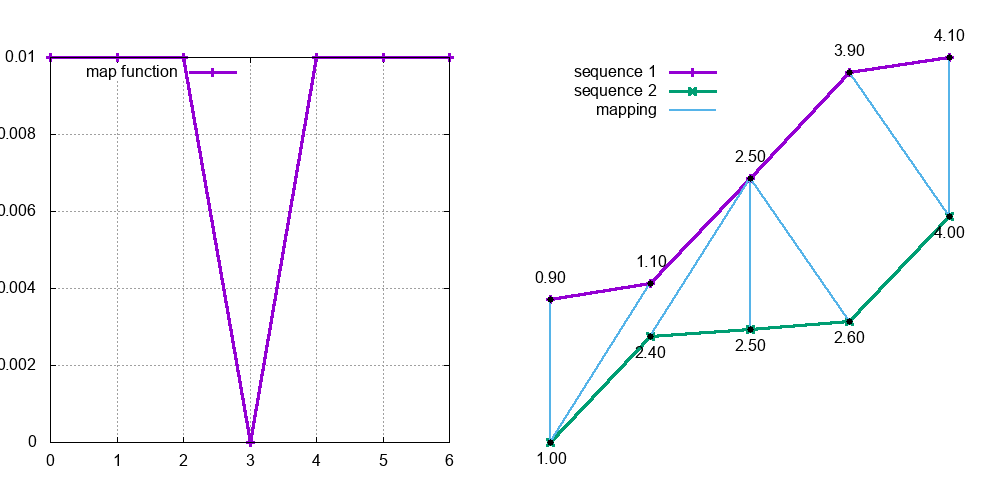
\includegraphics[scale=1.2, width=0.9\textwidth, height=0.425\textwidth]{simple}
        $$M(X, Y) = 0.00857143$$
    \end{figure}

    \item $X = \{1,\ 3.4,\ 8,\ 3.6,\ 1\}$, $Y = \{3.5,\ 9,\ 2.8\}$

    \begin{figure}[h]
        \centering
        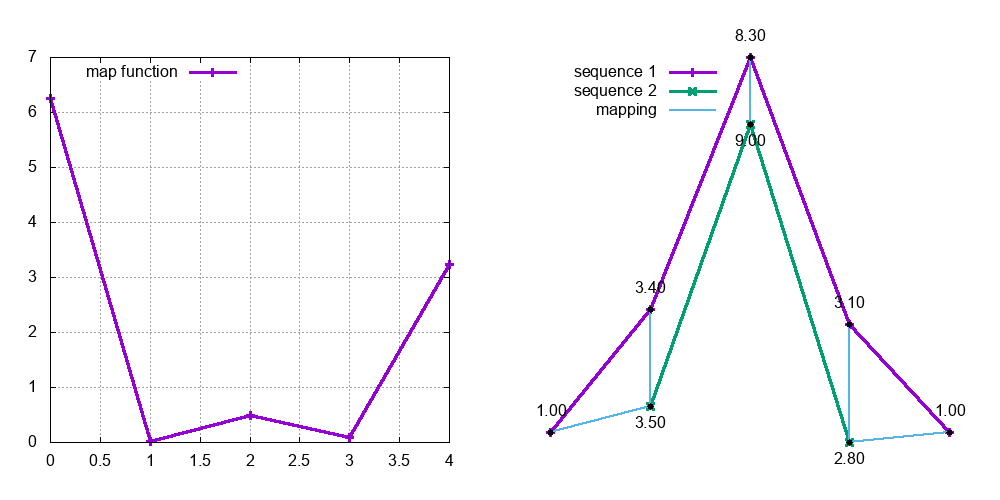
\includegraphics[scale=1.2, width=0.9\textwidth, height=0.425\textwidth]{unequal}
        $$M(X, Y) = 2.016$$
    \end{figure}

\newpage

    \item $X = \sin(x)$ на отрезке [0, 5], $Y = \sin(6x)$ на отрезке [0, 1]

    \begin{figure}[h]
        \centering
        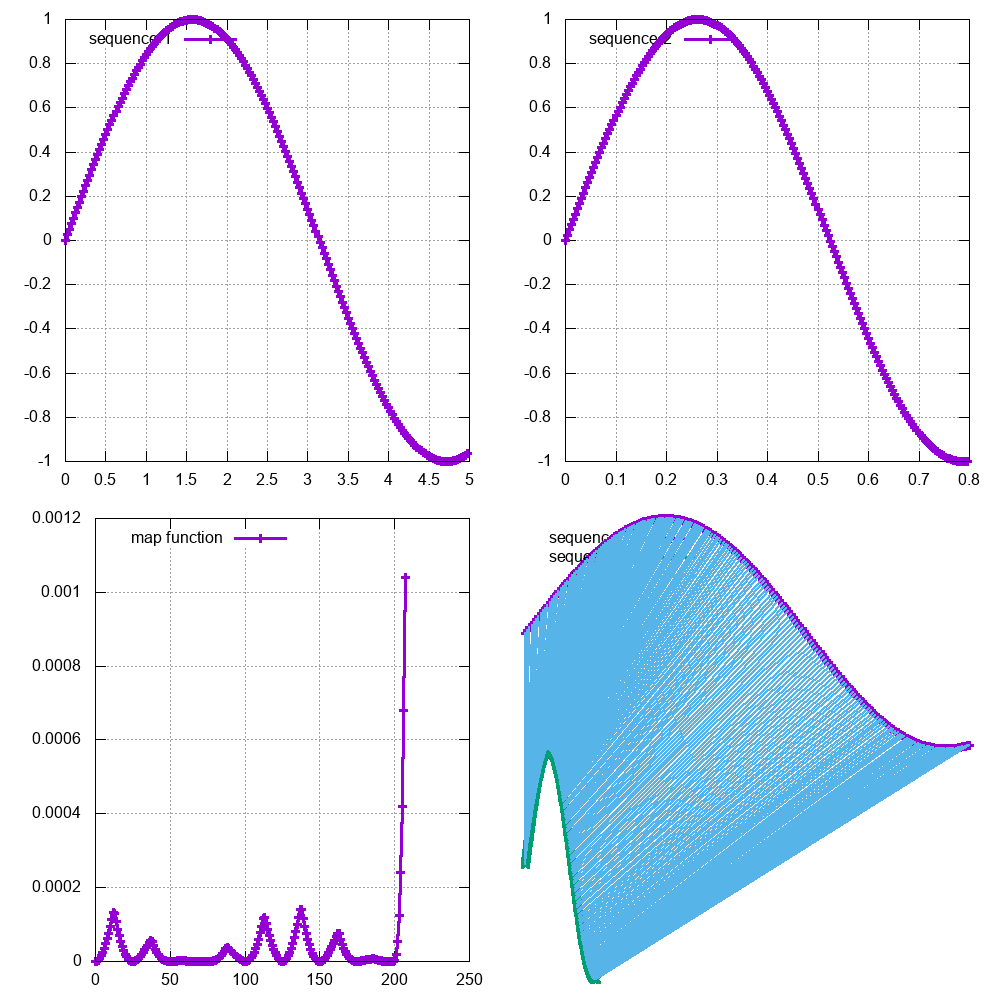
\includegraphics[scale=1.2, width=0.9\textwidth, height=0.8\textwidth]{sin}
        $$M(X, Y) = 3.69459e-05$$
    \end{figure}

    Заметим резкое возрастание функционала в конце. Это связано с тем,
    что после того как нашлось идеальное сопоставление $n$ точек первой последовательности
    в $k < n$ точек второй последовательности все остальные $n - k$ точек первой
    последовательности начали сопоставляться с последней точкой второй.
    Рассмотрим эту проблему далее в разделе Проблемы.

\newpage

    \item $$X = \exp(-\frac{x}{2})*( \sin(10*x*\cos(x))) \text{ на отрезке } [0, 5]$$
          $$Y = 1.2 \exp(-\frac{x+1}{2})*( \sin(10*(x+1)*\cos(x+1))) \text{ на отрезке } [0, 1]$$

    \begin{figure}[h]
        \centering
        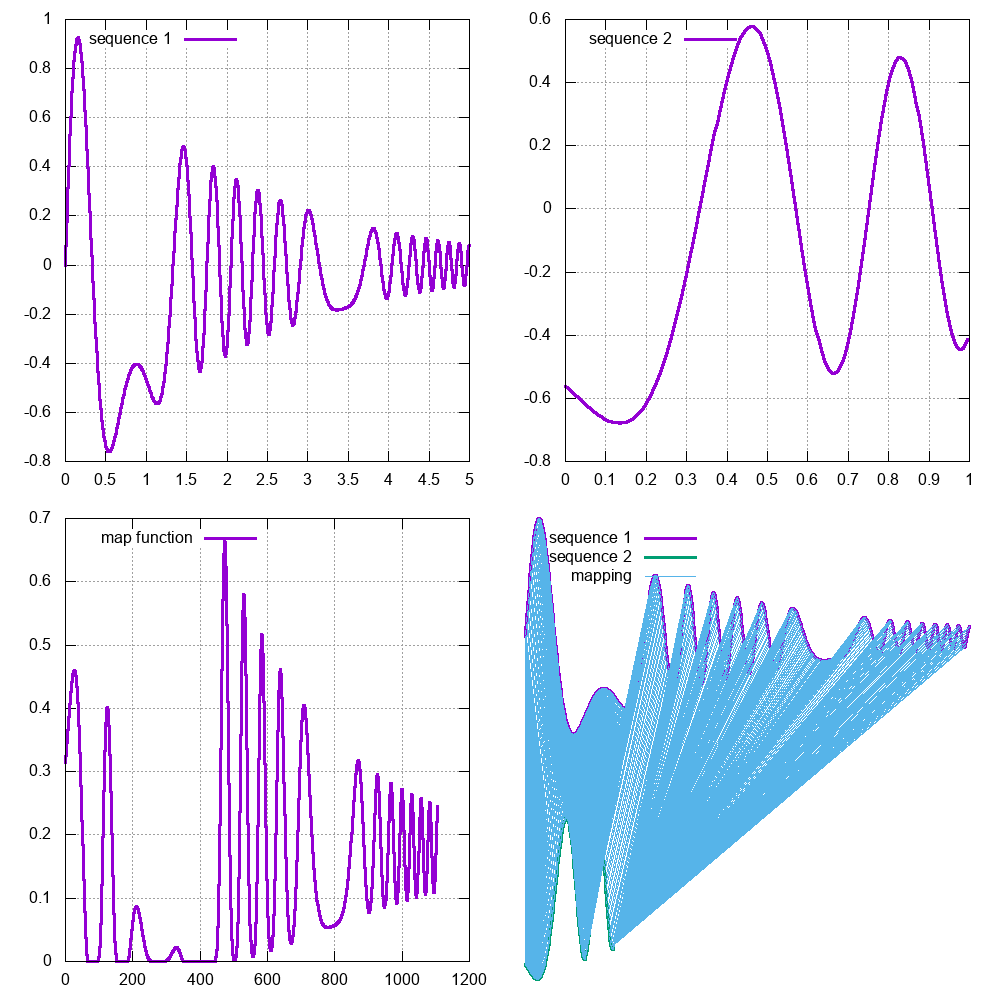
\includegraphics[scale=1.2, width=0.9\textwidth, height=0.8\textwidth]{cont1}
        $$M(X, Y) = 0.145174$$
    \end{figure}

    На данном примере наш алгоритм показал не совсем ожидаемый результат.
    В самом начале образовался ``веер``.
    То есть большая часть первой последовательности отобразилась в одну
    точку второй. Иначе говоря $y_j \mapsto {x_i,\ldots,x_{i+k}}$. Почему так произошло?
    Посмотрим подробнее в следующем разделе.

\end{enumerate}

\newpage
\subsection{Проблемы}

\subsubsection{Разные длины последовательностей}
     В третьем примере мы столкнулись с тем, что если в одной из последовательностей,
     допустим $X = (x_1, \ldots, x_n)$, количество элементов больше, чем в другой $Y = (y_1, \ldots,y_m)$,
     то есть $n > m$, то все $n - m$ элементов первой последовательности будут отражаться в последний
     элемент второй последовательности.

     \textbf{Возможное решение:} Довольно простое. Вместо того, чтобы идти по краю таблицы в правый
     нижний угол, будем обрывать алгоритм как только достигнем конца одной из последовательности.

    \textbf{Изменение в реализации:}
    \begin{lstlisting}
mapping_t map(const FloatingTable& table) {
    mapping_t result; std::array<double, 3> next;
    for (size_t i=0, j=0; i<table.nrows() && j<table.ncols();) {
        result.emplace_back(i, j);
        if (i+1 == table.nrows()) break;
        if (j+1 == table.ncols()) break;
        next = {
            table.at(i+1,j+1), table.at(i+1,j), table.at(i,j+1)
        };
        auto min_pos = std::min_element(next.begin(), next.end());
        if (min_pos == next.begin())
            i++, j++;
        else if (min_pos == std::next(next.begin()))
            i++;
        else
            j++;
    }
    return mapping_t;
}
    \end{lstlisting}


    \begin{figure}[h]
        \centering
        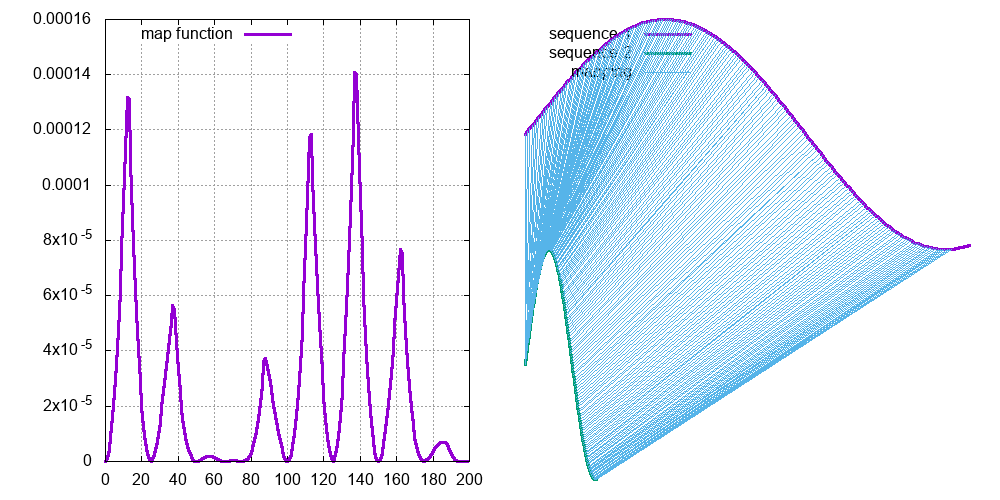
\includegraphics[scale=1.2, width=0.8\textwidth, height=0.4\textwidth]{sin2}
        $$M(X, Y) = 2.5505e-05$$
    \end{figure}

\newpage
\subsubsection{Множественные сопоставления одной точке}
    Посмотрим чему соответствует ``веер``, опираясь на замечание
    из Введения в алгоритм:

    \begin{center}
        \begin{tikzpicture}[
            ele/.style={fill=black,minimum width=.8pt,inner sep=1pt},
            baseline=(current bounding box.center)
        ]
            \node[ele,label=above:$x_0$]     (a0)   at (-6,1) {};
            \node[ele,label=above:$x_{j}$]   (aj)   at (-4.5,1) {};
            \node[ele]   (aj1)   at (-2,1) {};
            \node[ele]   (aj2)   at (-1,1) {};
            \node[ele]   (aj3)   at (0,1) {};
            \node[ele,label=above:$x_n$] (an) at (1,1) {};

            \node[ele,label=below:$y_0$]     (b0)   at (-6,0) {};
            \node[ele,label=below:$y_{i}$]   (bi)   at (-4, 0) {};
            \node[ele]   (bi0)   at (-3.75,0) {};
            \node[ele]   (bi1)   at (-3.5,0)  {};
            \node[ele]   (bi2)   at (-3.25,0) {};
            \node[ele]   (bi3)   at (-3,0) {};
            \node[ele]   (bi4)   at (-2.75,0) {};
            \node[ele,label=below:$y_{i+k}$] (bik)  at (-2.5, 0) {};
            \node[ele,label=below:$y_n$]     (bn)   at (0, 0) {};

            \begin{scope}[ultra thick,shorten <=2,shorten >=2]
                \draw (aj)   -- (bi);
                \draw (aj)   -- (bi0);
                \draw (aj)   -- (bi1);
                \draw (aj)   -- (bi2);
                \draw (aj)   -- (bi3);
                \draw (aj)   -- (bi4);
                \draw (aj)   -- (bik);
            \end{scope}
        \end{tikzpicture}
        $\Leftrightarrow$
        \begin{tikzpicture}[matr/.style={
            matrix of nodes,
            row sep=-\pgflinewidth,
            column sep=-\pgflinewidth,
            nodes={draw, text width=3.6em,align=center},
            text depth=1.25ex,
            text height=2.5ex,
            text width=1.5ex,
            nodes in empty cells
        },
        baseline=(current bounding box.center)]
        \matrix (m) [matr] {
                     & $\ldots$   & $x_j$   & $\ldots$ \\
            $\ldots$  &  \ldots   &  \ldots    &  \ldots  \\
            $y_i$     &  \ldots   &  |[fill=red!15!]|\ldots    &  \ldots  \\
            $\ldots$  &  \ldots   &  |[fill=red!15!]|\ldots    &  \ldots  \\
            $y_{i+k}$ &  \ldots   &  |[fill=red!15!]|\ldots    &  \ldots  \\
            $\ldots$  &  \ldots   &  \ldots    &  \ldots  \\
        };
        \end{tikzpicture}
    \end{center}

    \textbf{Вывод:} алгоритм жадно находит подходящее значение в таблице,
    которое дает наименьший вклад в функционал и не пытается смотреть на
    другие, возможно более подходящие значения.

    \textbf{Возможное решение:} Введем штрафы для нашего алгоритма таким
    образом:
    \begin{enumerate}
        \item Штраф за передвижение по столбцу $\alpha$ и строке $\beta$ равен 1.
        \item При выборе позиции перехода рассматриваем следующие значения:
            $\alpha * c_{i, j+1}$, $c_{j+1,i+1}, \beta * c_{i+1, j}$, где $c_{i',j'}$ -
            значение в ячейке $(i', j')$.
        \item Если подходящий элемент находится на следующей строке, то инкрементируем $\beta$,
            если на следующем столбце, то инкрементируем $\alpha$,
            если подходящий элемент лежит на диагонали, то $\alpha = \beta = 1$.
    \end{enumerate}

\newpage
    \textbf{Изменение в реализации:}
    \begin{lstlisting}
mapping_t map(const FloatingTable& table) {
    mapping_t result; std::array<double, 3> next;
    size_t row_penalty = 1, column_penalty = 1;
    for (size_t i=0, j=0; i<table.nrows() && j<table.ncols();) {
        result.emplace_back(i, j);
        if (i+1 == table.nrows()) break;
        if (j+1 == table.ncols()) break;
        next = {
            table.at(i+1,j+1),
            row_penalty * table.at(i+1,j),
            column_penalty * table.at(i,j+1)
        };
        auto min_pos = std::min_element(next.begin(), next.end());
        if (min_pos == next.begin())
            row_penalty = column_penalty = 1, i++, j++;
        else if (min_pos == std::next(next.begin()))
            i++, row_penalty++;
        else
            j++, column_penalty++;
    }
    return mapping_t;
}
    \end{lstlisting}

    \begin{figure}[h]
        \centering
        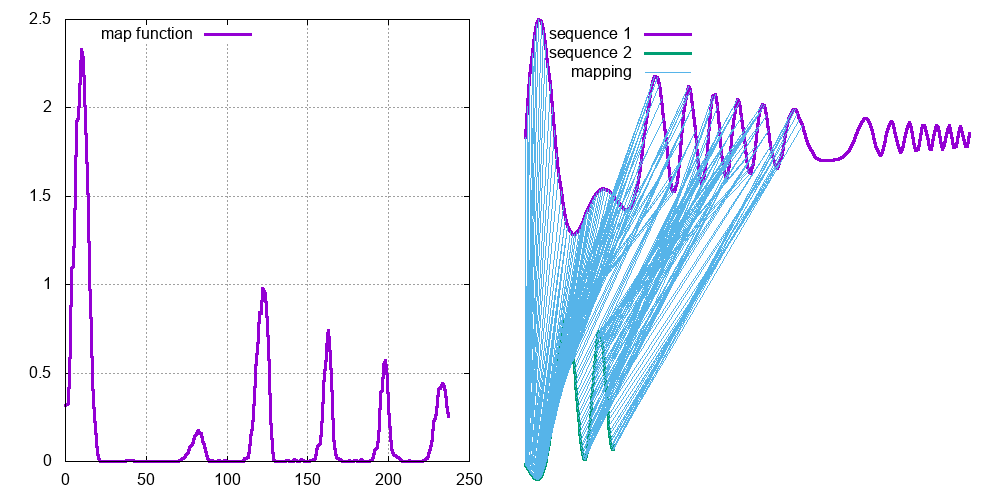
\includegraphics[scale=1.2, width=0.8\textwidth, height=0.4\textwidth]{cont2}
        $$M(X, Y) = 0.190666$$
    \end{figure}

\newpage
\subsubsection{Добавление первого элемента таблицы}
    Рассмотрим следующий пример

    \begin{figure}[h]
        \centering
        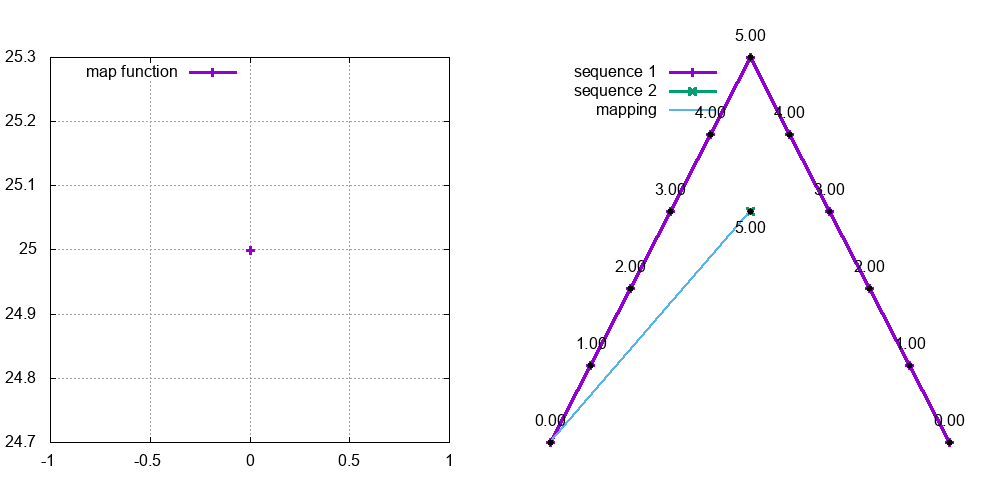
\includegraphics[scale=1.2, width=0.8\textwidth, height=0.4\textwidth]{problem3}
        $$M(X, Y) = 25$$
    \end{figure}

    Из-за того, что наш алгоритм начинает обход по таблице с левого верхнего угла и заканчивает работу
    тогда, когда хотя бы по одной из последовательностей закончится обход, мы получаем большое значение функционала.
    Нам бы хотелось, чтобы точка 5 второй последовательности из данного примера сопоставилась с соответсвующей
    ей точкой 5 из первой последовательности.

    \textbf{Возможное решение}: Давайте попробуем начинать наш алгоритм с поиска элемента второй
    последовательности такого, что наш функционал является минимальным.

    \textbf{Изменение в реализации:}
    \begin{lstlisting}
class FloatingTable {
 public:
    FloatingTable(const Sequence& BiggerSequence,
                  const Sequence& SmallerSequence)
        : _rows(BiggerSequence.size())
        , _columns(SmallerSequence.size())
        , _table(std::make_unique<uint32_t[]>(_rows * _columns)) {
        if (BiggerSequence.size() < SmallerSequence.size())
            throw std::runtime_error("Incorrect sizes");
        /* ... */
    }

    const double* begin() const
        { return _table.get(); }
    const double* end()   const
        { return _table.get() + _rows * _columns; }

 /* ... */
};
    \end{lstlisting}

\newpage

    \begin{lstlisting}
mapping_t map(const FloatingTable& table) {
    /* ... */
    auto pos = std::min_element(
        table.begin(), table.begin() + table.ncolumns()
    );
    size_t i = 0, j = (pos - table.begin());

    for (; i<table.nrows() && j<table.ncols();) {
        /* ... */
    }
    return result;
}
    \end{lstlisting}

    Посмотрим снова на приведенный пример:

    \begin{figure}[h]
        \centering
        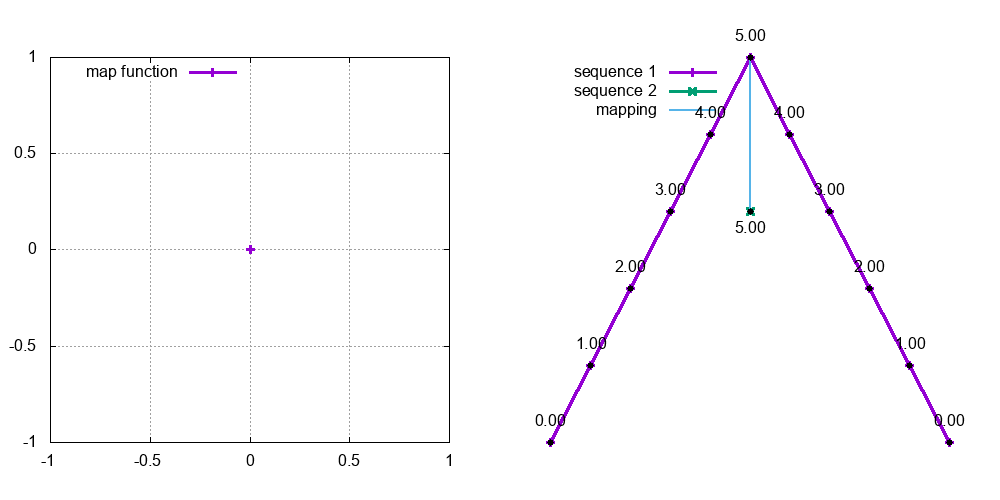
\includegraphics[scale=1.2, width=0.6\textwidth, height=0.3\textwidth]{solve3}
        $$M(X, Y) = 0$$
    \end{figure}

    Заметно улучшение. Давайте посмотрим на другие примеры:

    \begin{figure}[h]
        \centering
        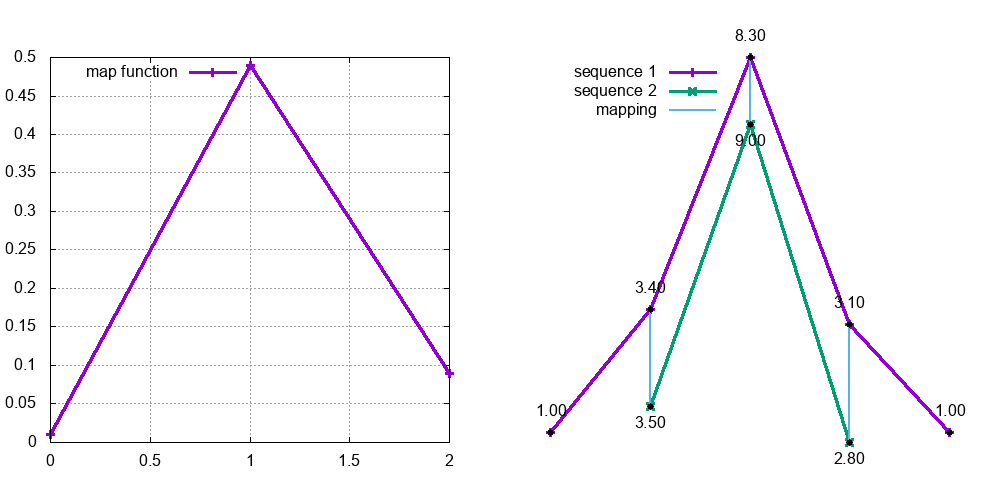
\includegraphics[scale=1.2, width=0.6\textwidth, height=0.3\textwidth]{new_unequal}
        $$M(X, Y) = 0.196667$$
    \end{figure}

    \newpage
    \begin{figure}[h]
        \centering
        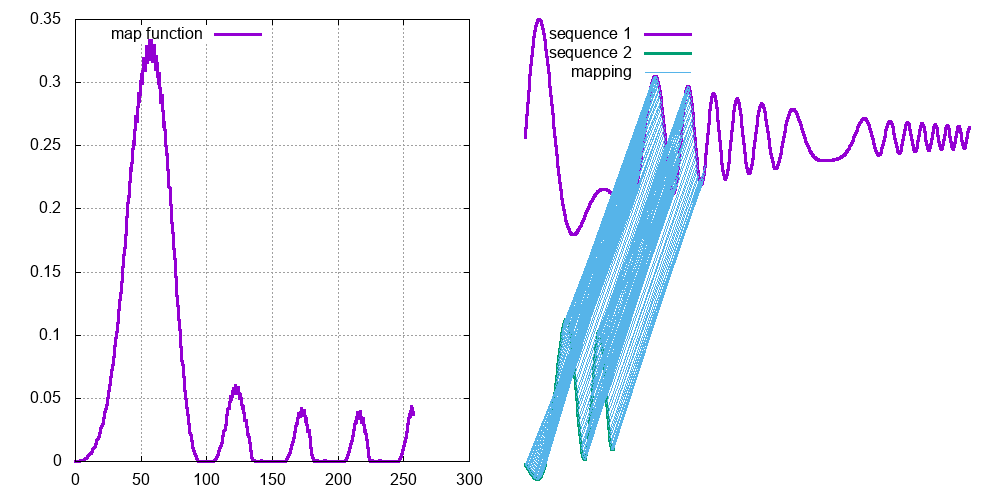
\includegraphics[scale=1.2, width=0.8\textwidth, height=0.4\textwidth]{cont3}
        $$M(X, Y) = 0.0575981$$
    \end{figure}

\subsection{Тестирование}

\begin{figure}[h]
    \centering
    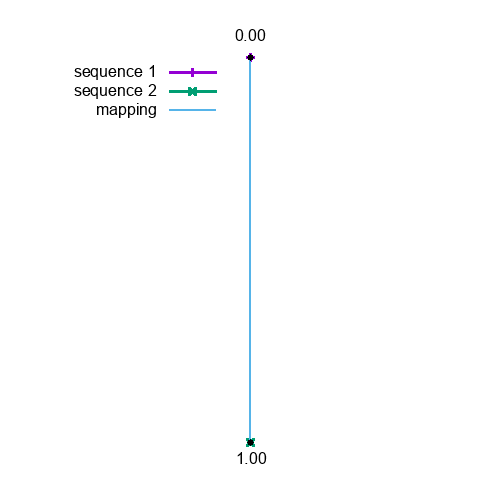
\includegraphics[width=0.45\textwidth, height=0.45\textwidth]{tests/one_to_one}
    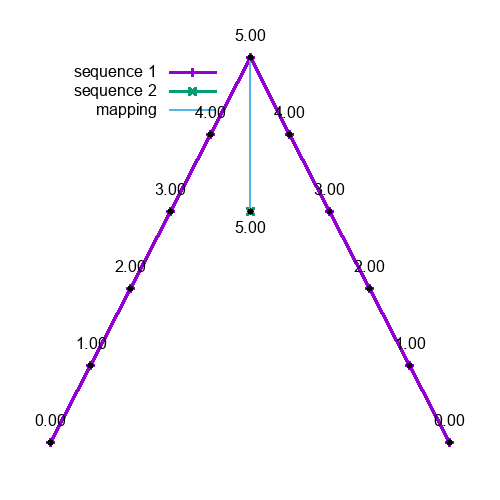
\includegraphics[width=0.45\textwidth, height=0.45\textwidth]{tests/one_to_all}
\end{figure}

\newpage

\begin{figure}[h]
    \centering
    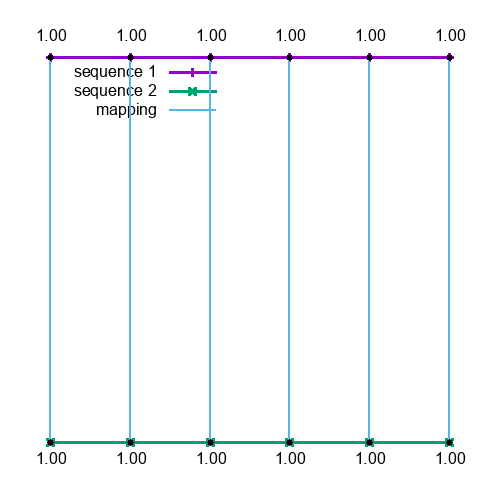
\includegraphics[width=0.45\textwidth, height=0.45\textwidth]{tests/constants}
    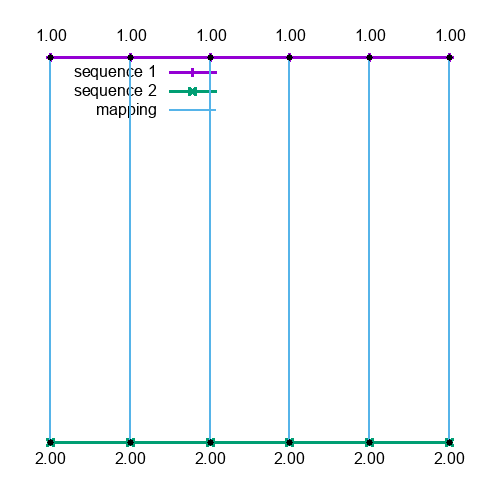
\includegraphics[width=0.45\textwidth, height=0.45\textwidth]{tests/diff_constants}
\end{figure}

\begin{figure}[h]
    \centering
    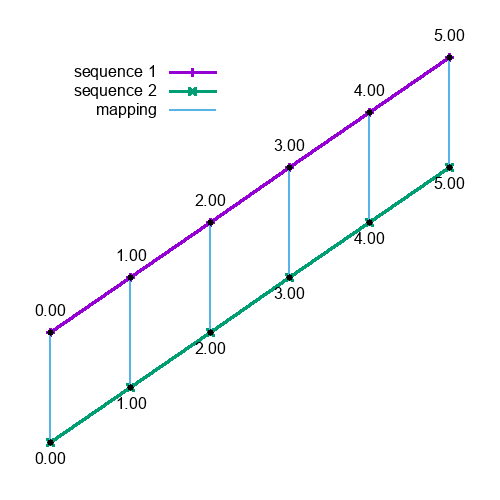
\includegraphics[width=0.45\textwidth, height=0.45\textwidth]{tests/incr}
    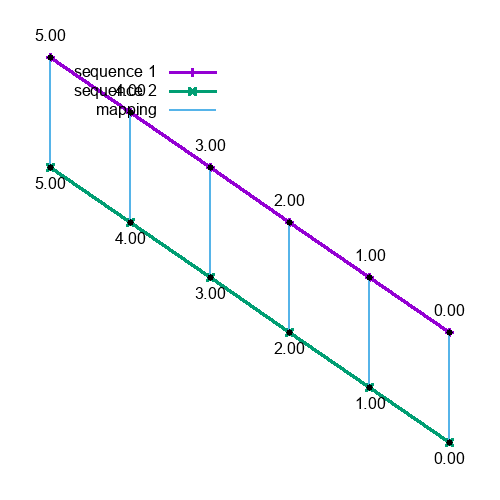
\includegraphics[width=0.45\textwidth, height=0.45\textwidth]{tests/decr}
\end{figure}

\newpage

\begin{figure}[h]
    \centering
    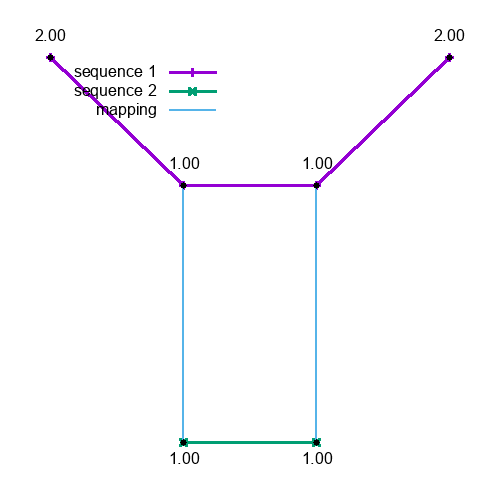
\includegraphics[width=0.3\textwidth, height=0.3\textwidth]{tests/misc1}
    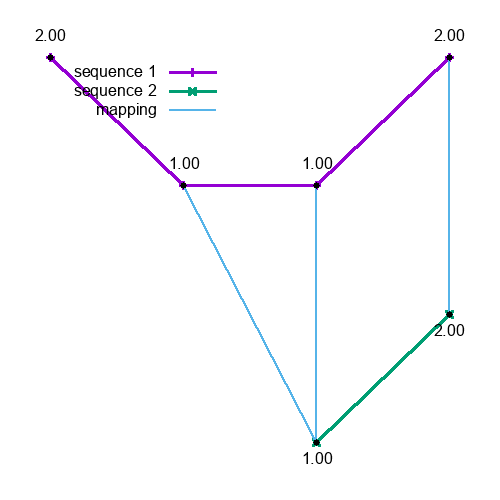
\includegraphics[width=0.3\textwidth, height=0.3\textwidth]{tests/misc2}
    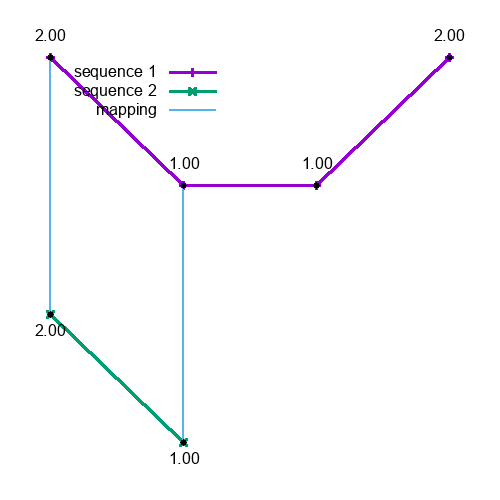
\includegraphics[width=0.3\textwidth, height=0.3\textwidth]{tests/misc3}
\end{figure}

\begin{figure}[h]
    \centering
    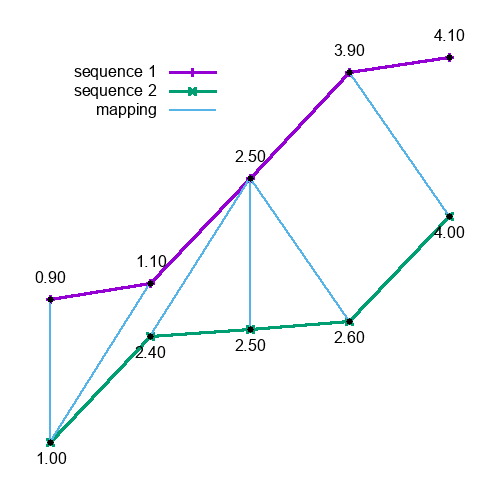
\includegraphics[width=0.34\textwidth, height=0.34\textwidth]{tests/simple}
    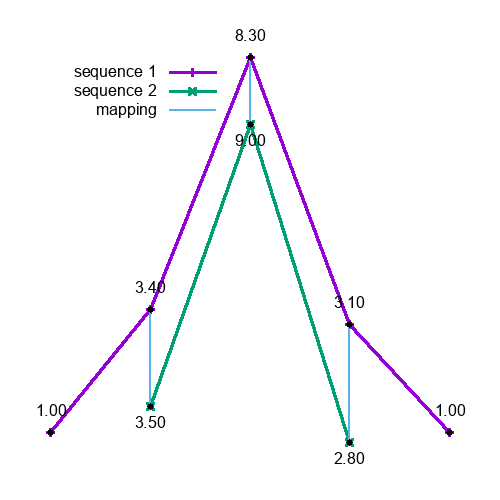
\includegraphics[width=0.34\textwidth, height=0.34\textwidth]{tests/unequal}
\end{figure}

\begin{figure}[h]
    \centering
    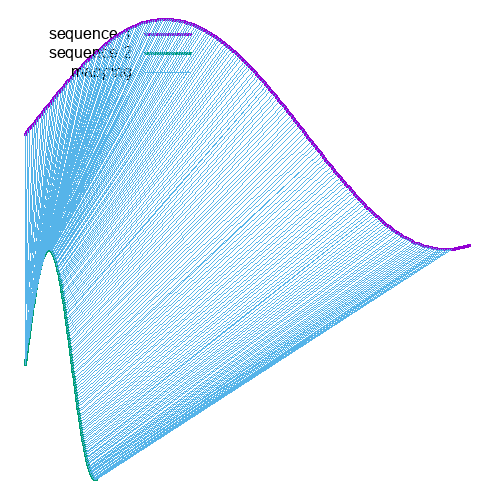
\includegraphics[width=0.35\textwidth, height=0.35\textwidth]{tests/sin}
    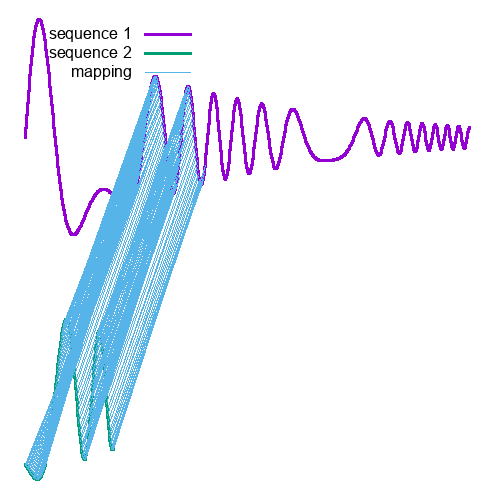
\includegraphics[width=0.35\textwidth, height=0.35\textwidth]{tests/cont}
\end{figure}



\end{document}